\documentclass[1p]{elsarticle_modified}
%\bibliographystyle{elsarticle-num}

%\usepackage[colorlinks]{hyperref}
%\usepackage{abbrmath_seonhwa} %\Abb, \Ascr, \Acal ,\Abf, \Afrak
\usepackage{amsfonts}
\usepackage{amssymb}
\usepackage{amsmath}
\usepackage{amsthm}
\usepackage{scalefnt}
\usepackage{amsbsy}
\usepackage{kotex}
\usepackage{caption}
\usepackage{subfig}
\usepackage{color}
\usepackage{graphicx}
\usepackage{xcolor} %% white, black, red, green, blue, cyan, magenta, yellow
\usepackage{float}
\usepackage{setspace}
\usepackage{hyperref}

\usepackage{tikz}
\usetikzlibrary{arrows}

\usepackage{multirow}
\usepackage{array} % fixed length table
\usepackage{hhline}

%%%%%%%%%%%%%%%%%%%%%
\makeatletter
\renewcommand*\env@matrix[1][\arraystretch]{%
	\edef\arraystretch{#1}%
	\hskip -\arraycolsep
	\let\@ifnextchar\new@ifnextchar
	\array{*\c@MaxMatrixCols c}}
\makeatother %https://tex.stackexchange.com/questions/14071/how-can-i-increase-the-line-spacing-in-a-matrix
%%%%%%%%%%%%%%%

\usepackage[normalem]{ulem}

\newcommand{\msout}[1]{\ifmmode\text{\sout{\ensuremath{#1}}}\else\sout{#1}\fi}
%SOURCE: \msout is \stkout macro in https://tex.stackexchange.com/questions/20609/strikeout-in-math-mode

\newcommand{\cancel}[1]{
	\ifmmode
	{\color{red}\msout{#1}}
	\else
	{\color{red}\sout{#1}}
	\fi
}

\newcommand{\add}[1]{
	{\color{blue}\uwave{#1}}
}

\newcommand{\replace}[2]{
	\ifmmode
	{\color{red}\msout{#1}}{\color{blue}\uwave{#2}}
	\else
	{\color{red}\sout{#1}}{\color{blue}\uwave{#2}}
	\fi
}

\newcommand{\Sol}{\mathcal{S}} %segment
\newcommand{\D}{D} %diagram
\newcommand{\A}{\mathcal{A}} %arc


%%%%%%%%%%%%%%%%%%%%%%%%%%%%%5 test

\def\sl{\operatorname{\textup{SL}}(2,\Cbb)}
\def\psl{\operatorname{\textup{PSL}}(2,\Cbb)}
\def\quan{\mkern 1mu \triangleright \mkern 1mu}

\theoremstyle{definition}
\newtheorem{thm}{Theorem}[section]
\newtheorem{prop}[thm]{Proposition}
\newtheorem{lem}[thm]{Lemma}
\newtheorem{ques}[thm]{Question}
\newtheorem{cor}[thm]{Corollary}
\newtheorem{defn}[thm]{Definition}
\newtheorem{exam}[thm]{Example}
\newtheorem{rmk}[thm]{Remark}
\newtheorem{alg}[thm]{Algorithm}

\newcommand{\I}{\sqrt{-1}}
\begin{document}

%\begin{frontmatter}
%
%\title{Boundary parabolic representations of knots up to 8 crossings}
%
%%% Group authors per affiliation:
%\author{Yunhi Cho} 
%\address{Department of Mathematics, University of Seoul, Seoul, Korea}
%\ead{yhcho@uos.ac.kr}
%
%
%\author{Seonhwa Kim} %\fnref{s_kim}}
%\address{Center for Geometry and Physics, Institute for Basic Science, Pohang, 37673, Korea}
%\ead{ryeona17@ibs.re.kr}
%
%\author{Hyuk Kim}
%\address{Department of Mathematical Sciences, Seoul National University, Seoul 08826, Korea}
%\ead{hyukkim@snu.ac.kr}
%
%\author{Seokbeom Yoon}
%\address{Department of Mathematical Sciences, Seoul National University, Seoul, 08826,  Korea}
%\ead{sbyoon15@snu.ac.kr}
%
%\begin{abstract}
%We find all boundary parabolic representation of knots up to 8 crossings.
%
%\end{abstract}
%\begin{keyword}
%    \MSC[2010] 57M25 
%\end{keyword}
%
%\end{frontmatter}

%\linenumbers
%\tableofcontents
%
\newcommand\colored[1]{\textcolor{white}{\rule[-0.35ex]{0.8em}{1.4ex}}\kern-0.8em\color{red} #1}%
%\newcommand\colored[1]{\textcolor{white}{ #1}\kern-2.17ex	\textcolor{white}{ #1}\kern-1.81ex	\textcolor{white}{ #1}\kern-2.15ex\color{red}#1	}

{\Large $\underline{12a_{0969}~(K12a_{0969})}$}

\setlength{\tabcolsep}{10pt}
\renewcommand{\arraystretch}{1.6}
\vspace{1cm}\begin{tabular}{m{100pt}>{\centering\arraybackslash}m{274pt}}
\multirow{5}{120pt}{
	\centering
	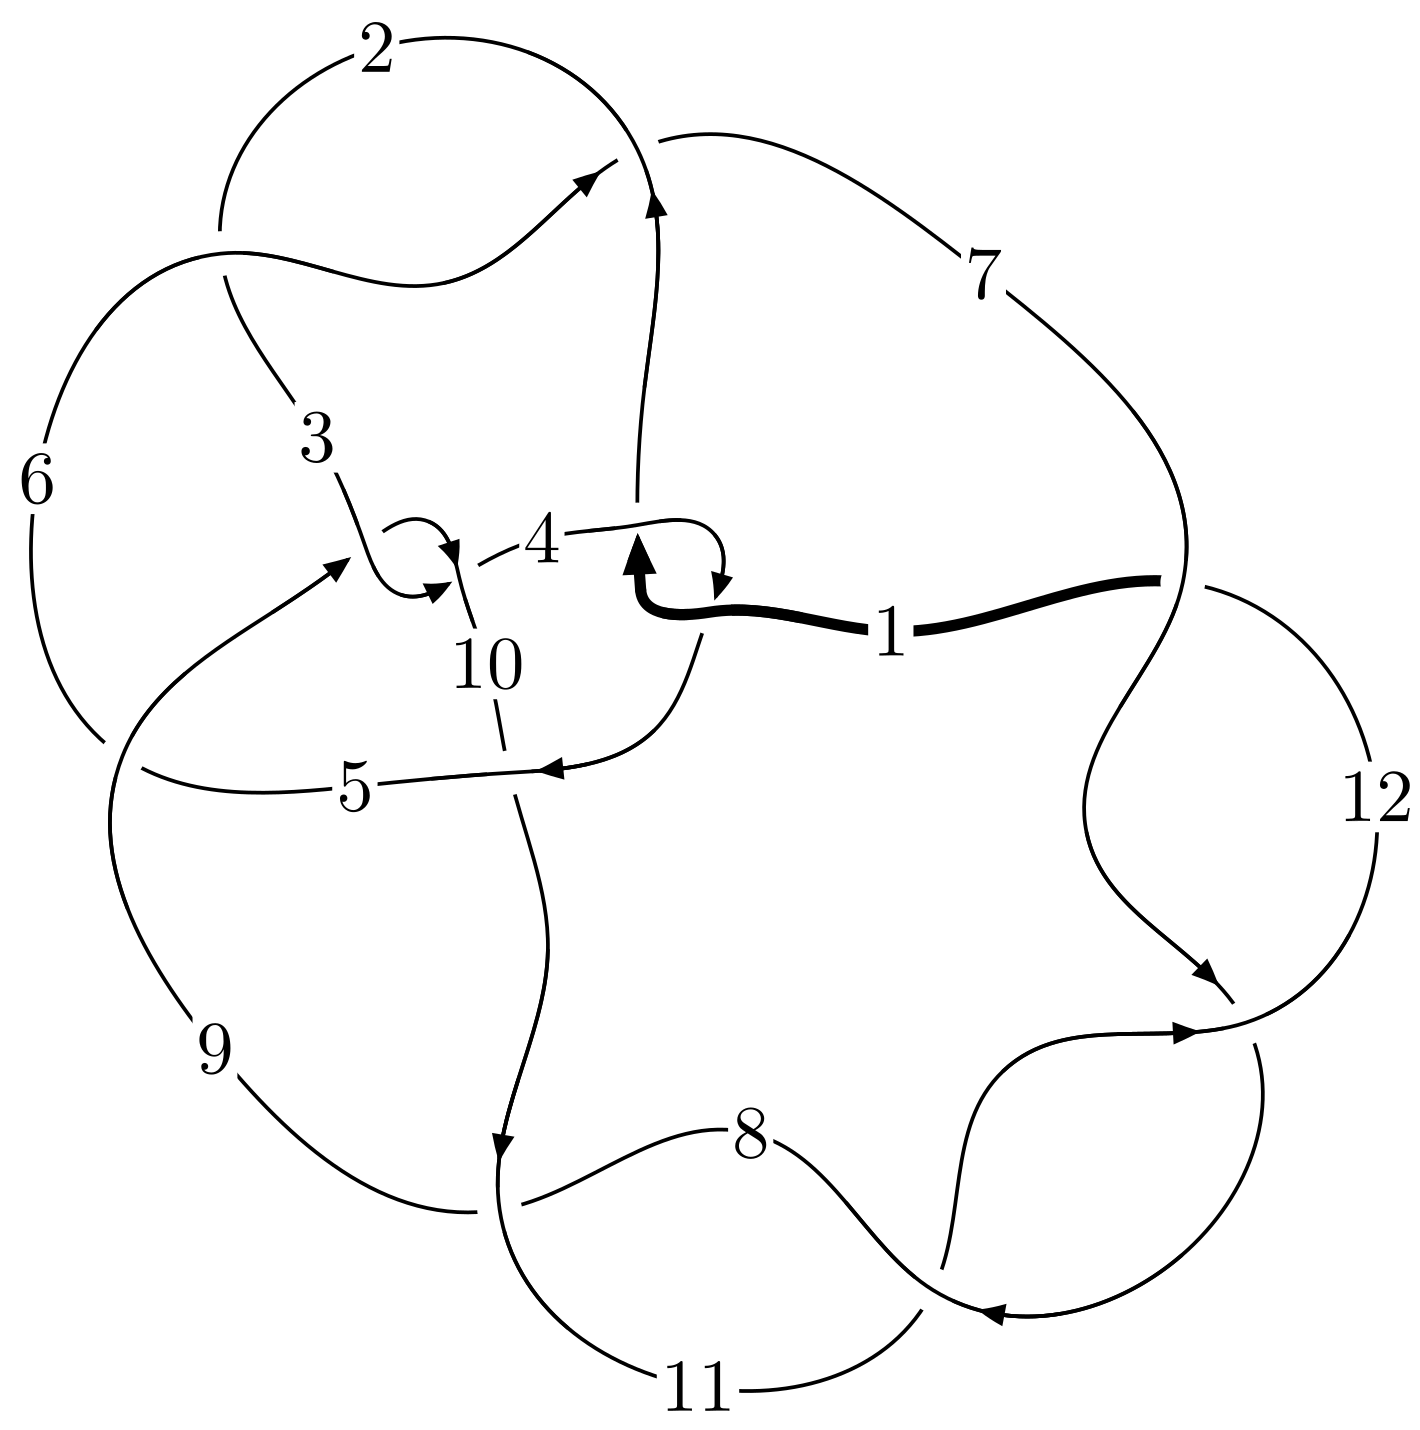
\includegraphics[width=112pt]{../../../GIT/diagram.site/Diagrams/png/1770_12a_0969.png}\\
\ \ \ A knot diagram\footnotemark}&
\allowdisplaybreaks
\textbf{Linearized knot diagam} \\
\cline{2-2}
 &
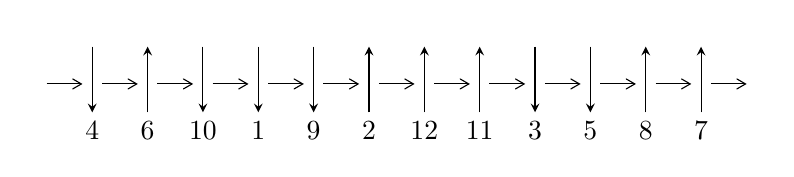
\begin{tikzpicture}[x=20pt, y=17pt]
	% nodes
	\node (C0) at (0, 0) {};
	\node (C1) at (1, 0) {};
	\node (C1U) at (1, +1) {};
	\node (C1D) at (1, -1) {4};

	\node (C2) at (2, 0) {};
	\node (C2U) at (2, +1) {};
	\node (C2D) at (2, -1) {6};

	\node (C3) at (3, 0) {};
	\node (C3U) at (3, +1) {};
	\node (C3D) at (3, -1) {10};

	\node (C4) at (4, 0) {};
	\node (C4U) at (4, +1) {};
	\node (C4D) at (4, -1) {1};

	\node (C5) at (5, 0) {};
	\node (C5U) at (5, +1) {};
	\node (C5D) at (5, -1) {9};

	\node (C6) at (6, 0) {};
	\node (C6U) at (6, +1) {};
	\node (C6D) at (6, -1) {2};

	\node (C7) at (7, 0) {};
	\node (C7U) at (7, +1) {};
	\node (C7D) at (7, -1) {12};

	\node (C8) at (8, 0) {};
	\node (C8U) at (8, +1) {};
	\node (C8D) at (8, -1) {11};

	\node (C9) at (9, 0) {};
	\node (C9U) at (9, +1) {};
	\node (C9D) at (9, -1) {3};

	\node (C10) at (10, 0) {};
	\node (C10U) at (10, +1) {};
	\node (C10D) at (10, -1) {5};

	\node (C11) at (11, 0) {};
	\node (C11U) at (11, +1) {};
	\node (C11D) at (11, -1) {8};

	\node (C12) at (12, 0) {};
	\node (C12U) at (12, +1) {};
	\node (C12D) at (12, -1) {7};
	\node (C13) at (13, 0) {};

	% arrows
	\draw[->,>={angle 60}]
	(C0) edge (C1) (C1) edge (C2) (C2) edge (C3) (C3) edge (C4) (C4) edge (C5) (C5) edge (C6) (C6) edge (C7) (C7) edge (C8) (C8) edge (C9) (C9) edge (C10) (C10) edge (C11) (C11) edge (C12) (C12) edge (C13) ;	\draw[->,>=stealth]
	(C1U) edge (C1D) (C2D) edge (C2U) (C3U) edge (C3D) (C4U) edge (C4D) (C5U) edge (C5D) (C6D) edge (C6U) (C7D) edge (C7U) (C8D) edge (C8U) (C9U) edge (C9D) (C10U) edge (C10D) (C11D) edge (C11U) (C12D) edge (C12U) ;
	\end{tikzpicture} \\
\hhline{~~} \\& 
\textbf{Solving Sequence} \\ \cline{2-2} 
 &
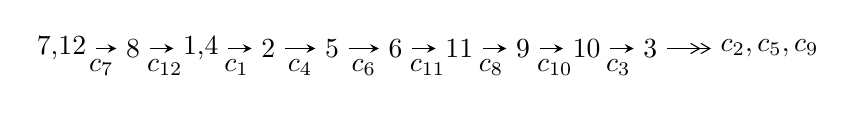
\begin{tikzpicture}[x=23pt, y=7pt]
	% node
	\node (A0) at (-1/8, 0) {7,12};
	\node (A1) at (1, 0) {8};
	\node (A2) at (33/16, 0) {1,4};
	\node (A3) at (25/8, 0) {2};
	\node (A4) at (33/8, 0) {5};
	\node (A5) at (41/8, 0) {6};
	\node (A6) at (49/8, 0) {11};
	\node (A7) at (57/8, 0) {9};
	\node (A8) at (65/8, 0) {10};
	\node (A9) at (73/8, 0) {3};
	\node (C1) at (1/2, -1) {$c_{7}$};
	\node (C2) at (3/2, -1) {$c_{12}$};
	\node (C3) at (21/8, -1) {$c_{1}$};
	\node (C4) at (29/8, -1) {$c_{4}$};
	\node (C5) at (37/8, -1) {$c_{6}$};
	\node (C6) at (45/8, -1) {$c_{11}$};
	\node (C7) at (53/8, -1) {$c_{8}$};
	\node (C8) at (61/8, -1) {$c_{10}$};
	\node (C9) at (69/8, -1) {$c_{3}$};
	\node (A10) at (11, 0) {$c_{2},c_{5},c_{9}$};

	% edge
	\draw[->,>=stealth]	
	(A0) edge (A1) (A1) edge (A2) (A2) edge (A3) (A3) edge (A4) (A4) edge (A5) (A5) edge (A6) (A6) edge (A7) (A7) edge (A8) (A8) edge (A9) ;
	\draw[->>,>={angle 60}]	
	(A9) edge (A10);
\end{tikzpicture} \\ 

\end{tabular} \\

\footnotetext{
The image of knot diagram is generated by the software ``\textbf{Draw programme}" developed by Andrew Bartholomew(\url{http://www.layer8.co.uk/maths/draw/index.htm\#Running-draw}), where we modified some parts for our purpose(\url{https://github.com/CATsTAILs/LinksPainter}).
}\phantom \\ \newline 
\centering \textbf{Ideals for irreducible components\footnotemark of $X_{\text{par}}$} 
 
\begin{align*}
I^u_{1}&=\langle 
-2.36400\times10^{116} u^{90}-5.03510\times10^{116} u^{89}+\cdots+7.67306\times10^{116} b+1.44976\times10^{118},\\
\phantom{I^u_{1}}&\phantom{= \langle  }-8.64013\times10^{119} u^{90}-2.09303\times10^{120} u^{89}+\cdots+5.34812\times10^{119} a+2.44441\times10^{121},\\
\phantom{I^u_{1}}&\phantom{= \langle  }u^{91}+3 u^{90}+\cdots+129 u+17\rangle \\
I^u_{2}&=\langle 
- u^{20}-2 u^{19}+\cdots+b-1,\;u^{21}- u^{20}+\cdots+a-7,\;u^{22}+2 u^{21}+\cdots+4 u+1\rangle \\
\\
\end{align*}
\raggedright * 2 irreducible components of $\dim_{\mathbb{C}}=0$, with total 113 representations.\\
\footnotetext{All coefficients of polynomials are rational numbers. But the coefficients are sometimes approximated in decimal forms when there is not enough margin.}
\newpage
\renewcommand{\arraystretch}{1}
\centering \section*{I. $I^u_{1}= \langle -2.36\times10^{116} u^{90}-5.04\times10^{116} u^{89}+\cdots+7.67\times10^{116} b+1.45\times10^{118},\;-8.64\times10^{119} u^{90}-2.09\times10^{120} u^{89}+\cdots+5.35\times10^{119} a+2.44\times10^{121},\;u^{91}+3 u^{90}+\cdots+129 u+17 \rangle$}
\flushleft \textbf{(i) Arc colorings}\\
\begin{tabular}{m{7pt} m{180pt} m{7pt} m{180pt} }
\flushright $a_{7}=$&$\begin{pmatrix}1\\0\end{pmatrix}$ \\
\flushright $a_{12}=$&$\begin{pmatrix}0\\u\end{pmatrix}$ \\
\flushright $a_{8}=$&$\begin{pmatrix}1\\- u^2\end{pmatrix}$ \\
\flushright $a_{1}=$&$\begin{pmatrix}u\\u\end{pmatrix}$ \\
\flushright $a_{4}=$&$\begin{pmatrix}1.61554 u^{90}+3.91359 u^{89}+\cdots-201.269 u-45.7060\\0.308091 u^{90}+0.656205 u^{89}+\cdots-77.7660 u-18.8941\end{pmatrix}$ \\
\flushright $a_{2}=$&$\begin{pmatrix}-0.882014 u^{90}-3.56244 u^{89}+\cdots-190.889 u-17.8701\\-0.381868 u^{90}-1.43162 u^{89}+\cdots+13.2970 u+4.16919\end{pmatrix}$ \\
\flushright $a_{5}=$&$\begin{pmatrix}1.03636 u^{90}+2.41410 u^{89}+\cdots-137.714 u-34.4014\\-0.271098 u^{90}-0.843285 u^{89}+\cdots-14.2107 u-7.58951\end{pmatrix}$ \\
\flushright $a_{6}=$&$\begin{pmatrix}1.62034 u^{90}+3.98249 u^{89}+\cdots-197.673 u-41.7998\\0.189004 u^{90}+0.362786 u^{89}+\cdots-70.2633 u-15.9802\end{pmatrix}$ \\
\flushright $a_{11}=$&$\begin{pmatrix}- u\\u^3+u\end{pmatrix}$ \\
\flushright $a_{9}=$&$\begin{pmatrix}u^2+1\\- u^4-2 u^2\end{pmatrix}$ \\
\flushright $a_{10}=$&$\begin{pmatrix}1.55728 u^{90}+3.97321 u^{89}+\cdots+15.5789 u-16.1108\\1.11898 u^{90}+2.89964 u^{89}+\cdots+76.9656 u-2.20818\end{pmatrix}$ \\
\flushright $a_{3}=$&$\begin{pmatrix}-0.354207 u^{90}-2.05941 u^{89}+\cdots-175.052 u-17.2076\\-0.735965 u^{90}-2.79677 u^{89}+\cdots-263.469 u-28.2611\end{pmatrix}$\\&\end{tabular}
\flushleft \textbf{(ii) Obstruction class $= -1$}\\~\\
\flushleft \textbf{(iii) Cusp Shapes $= 3.24325 u^{90}+10.4665 u^{89}+\cdots+642.496 u+57.8550$}\\~\\
\newpage\renewcommand{\arraystretch}{1}
\flushleft \textbf{(iv) u-Polynomials at the component}\newline \\
\begin{tabular}{m{50pt}|m{274pt}}
Crossings & \hspace{64pt}u-Polynomials at each crossing \\
\hline $$\begin{aligned}c_{1},c_{4}\end{aligned}$$&$\begin{aligned}
&u^{91}-5 u^{90}+\cdots-53 u+37
\end{aligned}$\\
\hline $$\begin{aligned}c_{2},c_{6}\end{aligned}$$&$\begin{aligned}
&u^{91}- u^{90}+\cdots+59093 u+8017
\end{aligned}$\\
\hline $$\begin{aligned}c_{3},c_{9}\end{aligned}$$&$\begin{aligned}
&u^{91}+u^{90}+\cdots+587 u+251
\end{aligned}$\\
\hline $$\begin{aligned}c_{5}\end{aligned}$$&$\begin{aligned}
&u^{91}+3 u^{90}+\cdots-4003055 u-530711
\end{aligned}$\\
\hline $$\begin{aligned}c_{7},c_{8},c_{11}\\c_{12}\end{aligned}$$&$\begin{aligned}
&u^{91}+3 u^{90}+\cdots+129 u+17
\end{aligned}$\\
\hline $$\begin{aligned}c_{10}\end{aligned}$$&$\begin{aligned}
&u^{91}- u^{90}+\cdots-79317 u+19177
\end{aligned}$\\
\hline
\end{tabular}\\~\\
\newpage\renewcommand{\arraystretch}{1}
\flushleft \textbf{(v) Riley Polynomials at the component}\newline \\
\begin{tabular}{m{50pt}|m{274pt}}
Crossings & \hspace{64pt}Riley Polynomials at each crossing \\
\hline $$\begin{aligned}c_{1},c_{4}\end{aligned}$$&$\begin{aligned}
&y^{91}+45 y^{90}+\cdots-55059 y-1369
\end{aligned}$\\
\hline $$\begin{aligned}c_{2},c_{6}\end{aligned}$$&$\begin{aligned}
&y^{91}+77 y^{90}+\cdots-1702552331 y-64272289
\end{aligned}$\\
\hline $$\begin{aligned}c_{3},c_{9}\end{aligned}$$&$\begin{aligned}
&y^{91}-63 y^{90}+\cdots+809421 y-63001
\end{aligned}$\\
\hline $$\begin{aligned}c_{5}\end{aligned}$$&$\begin{aligned}
&y^{91}-49 y^{90}+\cdots+8286890991737 y-281654165521
\end{aligned}$\\
\hline $$\begin{aligned}c_{7},c_{8},c_{11}\\c_{12}\end{aligned}$$&$\begin{aligned}
&y^{91}+113 y^{90}+\cdots-12021 y-289
\end{aligned}$\\
\hline $$\begin{aligned}c_{10}\end{aligned}$$&$\begin{aligned}
&y^{91}-29 y^{90}+\cdots+8475331727 y-367757329
\end{aligned}$\\
\hline
\end{tabular}\\~\\
\newpage\flushleft \textbf{(vi) Complex Volumes and Cusp Shapes}
$$\begin{array}{c|c|c}  
\text{Solutions to }I^u_{1}& \I (\text{vol} + \sqrt{-1}CS) & \text{Cusp shape}\\
 \hline 
\begin{aligned}
u &= \phantom{-}0.253030 + 1.006480 I \\
a &= -0.561408 + 0.901795 I \\
b &= -0.239624 + 0.297217 I\end{aligned}
 & -4.37050 + 2.04930 I & \phantom{-0.000000 } 0 \\ \hline\begin{aligned}
u &= \phantom{-}0.253030 - 1.006480 I \\
a &= -0.561408 - 0.901795 I \\
b &= -0.239624 - 0.297217 I\end{aligned}
 & -4.37050 - 2.04930 I & \phantom{-0.000000 } 0 \\ \hline\begin{aligned}
u &= -0.382221 + 0.872059 I \\
a &= -0.78902 - 1.24391 I \\
b &= \phantom{-}0.134758 - 0.340393 I\end{aligned}
 & -8.78899 - 6.69200 I & \phantom{-0.000000 } 0 \\ \hline\begin{aligned}
u &= -0.382221 - 0.872059 I \\
a &= -0.78902 + 1.24391 I \\
b &= \phantom{-}0.134758 + 0.340393 I\end{aligned}
 & -8.78899 + 6.69200 I & \phantom{-0.000000 } 0 \\ \hline\begin{aligned}
u &= -0.592298 + 0.866037 I \\
a &= \phantom{-}1.56047 + 0.34982 I \\
b &= \phantom{-}1.01433 + 1.56620 I\end{aligned}
 & -6.4664 - 13.2635 I & \phantom{-0.000000 } 0 \\ \hline\begin{aligned}
u &= -0.592298 - 0.866037 I \\
a &= \phantom{-}1.56047 - 0.34982 I \\
b &= \phantom{-}1.01433 - 1.56620 I\end{aligned}
 & -6.4664 + 13.2635 I & \phantom{-0.000000 } 0 \\ \hline\begin{aligned}
u &= \phantom{-}0.630431 + 0.846412 I \\
a &= \phantom{-}1.59404 - 0.38714 I \\
b &= \phantom{-}1.09526 - 1.46656 I\end{aligned}
 & -2.07560 + 6.94469 I & \phantom{-0.000000 } 0 \\ \hline\begin{aligned}
u &= \phantom{-}0.630431 - 0.846412 I \\
a &= \phantom{-}1.59404 + 0.38714 I \\
b &= \phantom{-}1.09526 + 1.46656 I\end{aligned}
 & -2.07560 - 6.94469 I & \phantom{-0.000000 } 0 \\ \hline\begin{aligned}
u &= -0.586607 + 0.740100 I \\
a &= \phantom{-}1.61009 + 0.36921 I \\
b &= \phantom{-}1.27345 + 1.42934 I\end{aligned}
 & -7.28302 - 0.64493 I & \phantom{-0.000000 } 0 \\ \hline\begin{aligned}
u &= -0.586607 - 0.740100 I \\
a &= \phantom{-}1.61009 - 0.36921 I \\
b &= \phantom{-}1.27345 - 1.42934 I\end{aligned}
 & -7.28302 + 0.64493 I & \phantom{-0.000000 } 0\\
 \hline 
 \end{array}$$\newpage$$\begin{array}{c|c|c}  
\text{Solutions to }I^u_{1}& \I (\text{vol} + \sqrt{-1}CS) & \text{Cusp shape}\\
 \hline 
\begin{aligned}
u &= -0.383140 + 0.844061 I \\
a &= -1.168540 - 0.674150 I \\
b &= -0.25614 - 1.62231 I\end{aligned}
 & -1.16419 - 6.82328 I & \phantom{-0.000000 } 0 \\ \hline\begin{aligned}
u &= -0.383140 - 0.844061 I \\
a &= -1.168540 + 0.674150 I \\
b &= -0.25614 + 1.62231 I\end{aligned}
 & -1.16419 + 6.82328 I & \phantom{-0.000000 } 0 \\ \hline\begin{aligned}
u &= \phantom{-}0.087898 + 1.089220 I \\
a &= \phantom{-}0.237486 - 0.259927 I \\
b &= -0.568773 + 0.022573 I\end{aligned}
 & -6.24220 + 0.44901 I & \phantom{-0.000000 } 0 \\ \hline\begin{aligned}
u &= \phantom{-}0.087898 - 1.089220 I \\
a &= \phantom{-}0.237486 + 0.259927 I \\
b &= -0.568773 - 0.022573 I\end{aligned}
 & -6.24220 - 0.44901 I & \phantom{-0.000000 } 0 \\ \hline\begin{aligned}
u &= \phantom{-}0.476782 + 0.744759 I \\
a &= -0.903469 + 0.549106 I \\
b &= -0.196827 + 1.373020 I\end{aligned}
 & \phantom{-}1.29917 + 3.07151 I & \phantom{-0.000000 } 0 \\ \hline\begin{aligned}
u &= \phantom{-}0.476782 - 0.744759 I \\
a &= -0.903469 - 0.549106 I \\
b &= -0.196827 - 1.373020 I\end{aligned}
 & \phantom{-}1.29917 - 3.07151 I & \phantom{-0.000000 } 0 \\ \hline\begin{aligned}
u &= \phantom{-}0.849193 + 0.173893 I \\
a &= -0.394385 + 0.552089 I \\
b &= \phantom{-}0.36794 + 1.42466 I\end{aligned}
 & \phantom{-}0.00220 - 2.00961 I & \phantom{-0.000000 } 0 \\ \hline\begin{aligned}
u &= \phantom{-}0.849193 - 0.173893 I \\
a &= -0.394385 - 0.552089 I \\
b &= \phantom{-}0.36794 - 1.42466 I\end{aligned}
 & \phantom{-}0.00220 + 2.00961 I & \phantom{-0.000000 } 0 \\ \hline\begin{aligned}
u &= -0.541487 + 1.036860 I \\
a &= -0.918599 - 0.986195 I \\
b &= -0.056278 - 0.887212 I\end{aligned}
 & -7.38711 + 3.94508 I & \phantom{-0.000000 } 0 \\ \hline\begin{aligned}
u &= -0.541487 - 1.036860 I \\
a &= -0.918599 + 0.986195 I \\
b &= -0.056278 + 0.887212 I\end{aligned}
 & -7.38711 - 3.94508 I & \phantom{-0.000000 } 0\\
 \hline 
 \end{array}$$\newpage$$\begin{array}{c|c|c}  
\text{Solutions to }I^u_{1}& \I (\text{vol} + \sqrt{-1}CS) & \text{Cusp shape}\\
 \hline 
\begin{aligned}
u &= -0.822520 + 0.067120 I \\
a &= -0.393774 - 0.210431 I \\
b &= \phantom{-}0.46423 - 1.43268 I\end{aligned}
 & -4.04382 + 8.57679 I & \phantom{-0.000000 } 0 \\ \hline\begin{aligned}
u &= -0.822520 - 0.067120 I \\
a &= -0.393774 + 0.210431 I \\
b &= \phantom{-}0.46423 + 1.43268 I\end{aligned}
 & -4.04382 - 8.57679 I & \phantom{-0.000000 } 0 \\ \hline\begin{aligned}
u &= -0.330329 + 0.695994 I \\
a &= -0.0350586 + 0.1285490 I \\
b &= -0.446342 - 0.727196 I\end{aligned}
 & -4.26951 - 2.65656 I & \phantom{-0.000000 } 0 \\ \hline\begin{aligned}
u &= -0.330329 - 0.695994 I \\
a &= -0.0350586 - 0.1285490 I \\
b &= -0.446342 + 0.727196 I\end{aligned}
 & -4.26951 + 2.65656 I & \phantom{-0.000000 } 0 \\ \hline\begin{aligned}
u &= \phantom{-}0.129252 + 0.718831 I \\
a &= \phantom{-}1.29791 + 0.61457 I \\
b &= \phantom{-}0.010107 - 0.407997 I\end{aligned}
 & -0.46804 + 2.58652 I & \phantom{-0.000000 } 0 \\ \hline\begin{aligned}
u &= \phantom{-}0.129252 - 0.718831 I \\
a &= \phantom{-}1.29791 - 0.61457 I \\
b &= \phantom{-}0.010107 + 0.407997 I\end{aligned}
 & -0.46804 - 2.58652 I & \phantom{-0.000000 } 0 \\ \hline\begin{aligned}
u &= \phantom{-}0.089930 + 0.719506 I \\
a &= -2.82227 + 0.94821 I \\
b &= -1.63207 + 1.65908 I\end{aligned}
 & -5.96732 + 3.75531 I & \phantom{-0.000000 } 0 \\ \hline\begin{aligned}
u &= \phantom{-}0.089930 - 0.719506 I \\
a &= -2.82227 - 0.94821 I \\
b &= -1.63207 - 1.65908 I\end{aligned}
 & -5.96732 - 3.75531 I & \phantom{-0.000000 } 0 \\ \hline\begin{aligned}
u &= \phantom{-}0.444816 + 0.571666 I \\
a &= -0.811182 - 0.626954 I \\
b &= -0.549553 + 1.222830 I\end{aligned}
 & -2.37455 + 4.94131 I & \phantom{-0.000000 } 0 \\ \hline\begin{aligned}
u &= \phantom{-}0.444816 - 0.571666 I \\
a &= -0.811182 + 0.626954 I \\
b &= -0.549553 - 1.222830 I\end{aligned}
 & -2.37455 - 4.94131 I & \phantom{-0.000000 } 0\\
 \hline 
 \end{array}$$\newpage$$\begin{array}{c|c|c}  
\text{Solutions to }I^u_{1}& \I (\text{vol} + \sqrt{-1}CS) & \text{Cusp shape}\\
 \hline 
\begin{aligned}
u &= \phantom{-}0.328418 + 1.300620 I \\
a &= -1.002710 + 0.773050 I \\
b &= -0.615435 + 0.689529 I\end{aligned}
 & -4.46238 + 2.26263 I & \phantom{-0.000000 } 0 \\ \hline\begin{aligned}
u &= \phantom{-}0.328418 - 1.300620 I \\
a &= -1.002710 - 0.773050 I \\
b &= -0.615435 - 0.689529 I\end{aligned}
 & -4.46238 - 2.26263 I & \phantom{-0.000000 } 0 \\ \hline\begin{aligned}
u &= \phantom{-}0.129039 + 1.345170 I \\
a &= \phantom{-}2.30985 - 0.06214 I \\
b &= \phantom{-}1.45692 - 0.23290 I\end{aligned}
 & -1.53404 + 3.13690 I & \phantom{-0.000000 } 0 \\ \hline\begin{aligned}
u &= \phantom{-}0.129039 - 1.345170 I \\
a &= \phantom{-}2.30985 + 0.06214 I \\
b &= \phantom{-}1.45692 + 0.23290 I\end{aligned}
 & -1.53404 - 3.13690 I & \phantom{-0.000000 } 0 \\ \hline\begin{aligned}
u &= -0.615697 + 0.164717 I \\
a &= -0.865139 - 0.742895 I \\
b &= \phantom{-}0.373819 - 1.212440 I\end{aligned}
 & -5.70084 - 3.45733 I & -4.35538 + 2.32913 I \\ \hline\begin{aligned}
u &= -0.615697 - 0.164717 I \\
a &= -0.865139 + 0.742895 I \\
b &= \phantom{-}0.373819 + 1.212440 I\end{aligned}
 & -5.70084 + 3.45733 I & -4.35538 - 2.32913 I \\ \hline\begin{aligned}
u &= -0.260413 + 0.575343 I \\
a &= -1.81516 + 0.48727 I \\
b &= -0.650904 - 1.158450 I\end{aligned}
 & -0.38808 - 3.24368 I & -2.30026 + 0. I\phantom{ +0.000000I} \\ \hline\begin{aligned}
u &= -0.260413 - 0.575343 I \\
a &= -1.81516 - 0.48727 I \\
b &= -0.650904 + 1.158450 I\end{aligned}
 & -0.38808 + 3.24368 I & -2.30026 + 0. I\phantom{ +0.000000I} \\ \hline\begin{aligned}
u &= \phantom{-}0.605745 + 0.178172 I \\
a &= \phantom{-}0.900250 + 0.429644 I \\
b &= \phantom{-}0.419929 - 1.077670 I\end{aligned}
 & \phantom{-}3.01354 + 0.62860 I & \phantom{-}6.07513 - 1.71881 I \\ \hline\begin{aligned}
u &= \phantom{-}0.605745 - 0.178172 I \\
a &= \phantom{-}0.900250 - 0.429644 I \\
b &= \phantom{-}0.419929 + 1.077670 I\end{aligned}
 & \phantom{-}3.01354 - 0.62860 I & \phantom{-}6.07513 + 1.71881 I\\
 \hline 
 \end{array}$$\newpage$$\begin{array}{c|c|c}  
\text{Solutions to }I^u_{1}& \I (\text{vol} + \sqrt{-1}CS) & \text{Cusp shape}\\
 \hline 
\begin{aligned}
u &= -0.354938 + 0.503980 I \\
a &= \phantom{-}1.58658 - 0.00995 I \\
b &= -0.125767 + 0.884945 I\end{aligned}
 & -0.096196 + 1.233880 I & -2.89346 + 1.13895 I \\ \hline\begin{aligned}
u &= -0.354938 - 0.503980 I \\
a &= \phantom{-}1.58658 + 0.00995 I \\
b &= -0.125767 - 0.884945 I\end{aligned}
 & -0.096196 - 1.233880 I & -2.89346 - 1.13895 I \\ \hline\begin{aligned}
u &= \phantom{-}0.516984 + 0.310035 I \\
a &= \phantom{-}1.54678 + 0.12545 I \\
b &= -0.346073 - 0.764503 I\end{aligned}
 & -1.62456 - 1.58941 I & -2.19411 - 0.24297 I \\ \hline\begin{aligned}
u &= \phantom{-}0.516984 - 0.310035 I \\
a &= \phantom{-}1.54678 - 0.12545 I \\
b &= -0.346073 + 0.764503 I\end{aligned}
 & -1.62456 + 1.58941 I & -2.19411 + 0.24297 I \\ \hline\begin{aligned}
u &= -0.039764 + 0.550957 I \\
a &= -3.59783 + 0.41411 I \\
b &= -0.878611 - 0.342232 I\end{aligned}
 & \phantom{-}0.43967 - 2.50241 I & -6.35136 + 5.68313 I \\ \hline\begin{aligned}
u &= -0.039764 - 0.550957 I \\
a &= -3.59783 - 0.41411 I \\
b &= -0.878611 + 0.342232 I\end{aligned}
 & \phantom{-}0.43967 + 2.50241 I & -6.35136 - 5.68313 I \\ \hline\begin{aligned}
u &= -0.04384 + 1.49074 I \\
a &= \phantom{-}1.238740 + 0.265818 I \\
b &= \phantom{-}0.343289 + 0.401998 I\end{aligned}
 & -6.54801 - 0.21182 I & \phantom{-0.000000 } 0 \\ \hline\begin{aligned}
u &= -0.04384 - 1.49074 I \\
a &= \phantom{-}1.238740 - 0.265818 I \\
b &= \phantom{-}0.343289 - 0.401998 I\end{aligned}
 & -6.54801 + 0.21182 I & \phantom{-0.000000 } 0 \\ \hline\begin{aligned}
u &= -0.506629 + 0.013297 I \\
a &= \phantom{-}0.635914 + 1.176010 I \\
b &= \phantom{-}0.085659 - 1.171430 I\end{aligned}
 & \phantom{-}1.39516 - 3.73965 I & \phantom{-}2.89170 + 5.40187 I \\ \hline\begin{aligned}
u &= -0.506629 - 0.013297 I \\
a &= \phantom{-}0.635914 - 1.176010 I \\
b &= \phantom{-}0.085659 + 1.171430 I\end{aligned}
 & \phantom{-}1.39516 + 3.73965 I & \phantom{-}2.89170 - 5.40187 I\\
 \hline 
 \end{array}$$\newpage$$\begin{array}{c|c|c}  
\text{Solutions to }I^u_{1}& \I (\text{vol} + \sqrt{-1}CS) & \text{Cusp shape}\\
 \hline 
\begin{aligned}
u &= -0.456972\phantom{ +0.000000I} \\
a &= \phantom{-}1.32803\phantom{ +0.000000I} \\
b &= -0.280726\phantom{ +0.000000I}\end{aligned}
 & -2.27036\phantom{ +0.000000I} & -2.15750\phantom{ +0.000000I} \\ \hline\begin{aligned}
u &= \phantom{-}0.220977 + 0.398435 I \\
a &= \phantom{-}0.697056 + 0.380194 I \\
b &= \phantom{-}0.104360 + 0.315206 I\end{aligned}
 & \phantom{-}0.003690 + 0.929769 I & \phantom{-}0.15778 - 7.14917 I \\ \hline\begin{aligned}
u &= \phantom{-}0.220977 - 0.398435 I \\
a &= \phantom{-}0.697056 - 0.380194 I \\
b &= \phantom{-}0.104360 - 0.315206 I\end{aligned}
 & \phantom{-}0.003690 - 0.929769 I & \phantom{-}0.15778 + 7.14917 I \\ \hline\begin{aligned}
u &= -0.199743 + 0.398483 I \\
a &= \phantom{-}1.67316 + 0.34201 I \\
b &= -0.234533 + 0.862944 I\end{aligned}
 & \phantom{-}0.072497 + 1.266220 I & -4.46493 - 2.74628 I \\ \hline\begin{aligned}
u &= -0.199743 - 0.398483 I \\
a &= \phantom{-}1.67316 - 0.34201 I \\
b &= -0.234533 - 0.862944 I\end{aligned}
 & \phantom{-}0.072497 - 1.266220 I & -4.46493 + 2.74628 I \\ \hline\begin{aligned}
u &= \phantom{-}0.10145 + 1.56912 I \\
a &= -1.34483 + 0.73744 I \\
b &= -0.81044 + 1.53567 I\end{aligned}
 & -9.60673 + 6.81055 I & \phantom{-0.000000 } 0 \\ \hline\begin{aligned}
u &= \phantom{-}0.10145 - 1.56912 I \\
a &= -1.34483 - 0.73744 I \\
b &= -0.81044 - 1.53567 I\end{aligned}
 & -9.60673 - 6.81055 I & \phantom{-0.000000 } 0 \\ \hline\begin{aligned}
u &= -0.09827 + 1.57654 I \\
a &= -1.18204 - 1.29658 I \\
b &= -1.08401 - 1.66241 I\end{aligned}
 & -11.94870 - 4.17333 I & \phantom{-0.000000 } 0 \\ \hline\begin{aligned}
u &= -0.09827 - 1.57654 I \\
a &= -1.18204 + 1.29658 I \\
b &= -1.08401 + 1.66241 I\end{aligned}
 & -11.94870 + 4.17333 I & \phantom{-0.000000 } 0 \\ \hline\begin{aligned}
u &= \phantom{-}0.00011 + 1.58693 I \\
a &= \phantom{-}0.948307 + 0.856943 I \\
b &= \phantom{-}0.423379 + 1.197460 I\end{aligned}
 & -6.99880 + 1.08422 I & \phantom{-0.000000 } 0\\
 \hline 
 \end{array}$$\newpage$$\begin{array}{c|c|c}  
\text{Solutions to }I^u_{1}& \I (\text{vol} + \sqrt{-1}CS) & \text{Cusp shape}\\
 \hline 
\begin{aligned}
u &= \phantom{-}0.00011 - 1.58693 I \\
a &= \phantom{-}0.948307 - 0.856943 I \\
b &= \phantom{-}0.423379 - 1.197460 I\end{aligned}
 & -6.99880 - 1.08422 I & \phantom{-0.000000 } 0 \\ \hline\begin{aligned}
u &= -0.04388 + 1.59590 I \\
a &= \phantom{-}0.08672 - 1.66738 I \\
b &= -0.17594 - 1.98522 I\end{aligned}
 & -11.93620 - 3.98067 I & \phantom{-0.000000 } 0 \\ \hline\begin{aligned}
u &= -0.04388 - 1.59590 I \\
a &= \phantom{-}0.08672 + 1.66738 I \\
b &= -0.17594 + 1.98522 I\end{aligned}
 & -11.93620 + 3.98067 I & \phantom{-0.000000 } 0 \\ \hline\begin{aligned}
u &= -0.06162 + 1.59587 I \\
a &= -1.80580 - 0.79874 I \\
b &= -1.06224 - 1.38386 I\end{aligned}
 & -7.94061 - 4.34595 I & \phantom{-0.000000 } 0 \\ \hline\begin{aligned}
u &= -0.06162 - 1.59587 I \\
a &= -1.80580 + 0.79874 I \\
b &= -1.06224 + 1.38386 I\end{aligned}
 & -7.94061 + 4.34595 I & \phantom{-0.000000 } 0 \\ \hline\begin{aligned}
u &= -0.042082 + 0.397737 I \\
a &= \phantom{-}0.24997 - 2.36679 I \\
b &= -0.78595 - 1.78034 I\end{aligned}
 & -4.81875 - 3.37599 I & -7.29184 - 1.97538 I \\ \hline\begin{aligned}
u &= -0.042082 - 0.397737 I \\
a &= \phantom{-}0.24997 + 2.36679 I \\
b &= -0.78595 + 1.78034 I\end{aligned}
 & -4.81875 + 3.37599 I & -7.29184 + 1.97538 I \\ \hline\begin{aligned}
u &= -0.00951 + 1.60358 I \\
a &= -2.57300 - 0.18687 I \\
b &= -1.47153 - 0.38335 I\end{aligned}
 & -7.18483 - 2.67195 I & \phantom{-0.000000 } 0 \\ \hline\begin{aligned}
u &= -0.00951 - 1.60358 I \\
a &= -2.57300 + 0.18687 I \\
b &= -1.47153 + 0.38335 I\end{aligned}
 & -7.18483 + 2.67195 I & \phantom{-0.000000 } 0 \\ \hline\begin{aligned}
u &= \phantom{-}0.03262 + 1.61996 I \\
a &= \phantom{-}0.792831 - 0.242520 I \\
b &= \phantom{-}0.200055 - 0.835980 I\end{aligned}
 & -8.56287 + 3.20352 I & \phantom{-0.000000 } 0\\
 \hline 
 \end{array}$$\newpage$$\begin{array}{c|c|c}  
\text{Solutions to }I^u_{1}& \I (\text{vol} + \sqrt{-1}CS) & \text{Cusp shape}\\
 \hline 
\begin{aligned}
u &= \phantom{-}0.03262 - 1.61996 I \\
a &= \phantom{-}0.792831 + 0.242520 I \\
b &= \phantom{-}0.200055 + 0.835980 I\end{aligned}
 & -8.56287 - 3.20352 I & \phantom{-0.000000 } 0 \\ \hline\begin{aligned}
u &= \phantom{-}0.13259 + 1.62867 I \\
a &= -1.24348 + 1.20206 I \\
b &= -0.72606 + 1.56533 I\end{aligned}
 & -6.82850 + 5.34807 I & \phantom{-0.000000 } 0 \\ \hline\begin{aligned}
u &= \phantom{-}0.13259 - 1.62867 I \\
a &= -1.24348 - 1.20206 I \\
b &= -0.72606 - 1.56533 I\end{aligned}
 & -6.82850 - 5.34807 I & \phantom{-0.000000 } 0 \\ \hline\begin{aligned}
u &= \phantom{-}0.02825 + 1.63775 I \\
a &= -2.88026 + 1.42748 I \\
b &= -2.20110 + 1.72105 I\end{aligned}
 & -14.2601 + 4.2220 I & \phantom{-0.000000 } 0 \\ \hline\begin{aligned}
u &= \phantom{-}0.02825 - 1.63775 I \\
a &= -2.88026 - 1.42748 I \\
b &= -2.20110 - 1.72105 I\end{aligned}
 & -14.2601 - 4.2220 I & \phantom{-0.000000 } 0 \\ \hline\begin{aligned}
u &= -0.18525 + 1.64009 I \\
a &= \phantom{-}2.56449 + 0.80433 I \\
b &= \phantom{-}1.93148 + 1.24752 I\end{aligned}
 & -15.3815 - 3.6242 I & \phantom{-0.000000 } 0 \\ \hline\begin{aligned}
u &= -0.18525 - 1.64009 I \\
a &= \phantom{-}2.56449 - 0.80433 I \\
b &= \phantom{-}1.93148 - 1.24752 I\end{aligned}
 & -15.3815 + 3.6242 I & \phantom{-0.000000 } 0 \\ \hline\begin{aligned}
u &= -0.10744 + 1.66260 I \\
a &= -0.254529 - 0.572722 I \\
b &= \phantom{-}0.135258 + 0.231828 I\end{aligned}
 & -17.5577 - 8.5967 I & \phantom{-0.000000 } 0 \\ \hline\begin{aligned}
u &= -0.10744 - 1.66260 I \\
a &= -0.254529 + 0.572722 I \\
b &= \phantom{-}0.135258 - 0.231828 I\end{aligned}
 & -17.5577 + 8.5967 I & \phantom{-0.000000 } 0 \\ \hline\begin{aligned}
u &= -0.10822 + 1.66536 I \\
a &= -1.23552 - 1.50937 I \\
b &= -0.60319 - 1.90161 I\end{aligned}
 & -9.88898 - 8.72775 I & \phantom{-0.000000 } 0\\
 \hline 
 \end{array}$$\newpage$$\begin{array}{c|c|c}  
\text{Solutions to }I^u_{1}& \I (\text{vol} + \sqrt{-1}CS) & \text{Cusp shape}\\
 \hline 
\begin{aligned}
u &= -0.10822 - 1.66536 I \\
a &= -1.23552 + 1.50937 I \\
b &= -0.60319 + 1.90161 I\end{aligned}
 & -9.88898 + 8.72775 I & \phantom{-0.000000 } 0 \\ \hline\begin{aligned}
u &= \phantom{-}0.18270 + 1.66545 I \\
a &= \phantom{-}2.28916 - 0.86051 I \\
b &= \phantom{-}1.58319 - 1.36510 I\end{aligned}
 & -10.6371 + 10.0743 I & \phantom{-0.000000 } 0 \\ \hline\begin{aligned}
u &= \phantom{-}0.18270 - 1.66545 I \\
a &= \phantom{-}2.28916 + 0.86051 I \\
b &= \phantom{-}1.58319 + 1.36510 I\end{aligned}
 & -10.6371 - 10.0743 I & \phantom{-0.000000 } 0 \\ \hline\begin{aligned}
u &= -0.17542 + 1.66854 I \\
a &= \phantom{-}2.17852 + 1.00647 I \\
b &= \phantom{-}1.46947 + 1.57996 I\end{aligned}
 & -15.1212 - 16.2518 I & \phantom{-0.000000 } 0 \\ \hline\begin{aligned}
u &= -0.17542 - 1.66854 I \\
a &= \phantom{-}2.17852 - 1.00647 I \\
b &= \phantom{-}1.46947 - 1.57996 I\end{aligned}
 & -15.1212 + 16.2518 I & \phantom{-0.000000 } 0 \\ \hline\begin{aligned}
u &= \phantom{-}0.08358 + 1.68225 I \\
a &= -0.225378 + 0.439636 I \\
b &= -0.032799 - 0.242739 I\end{aligned}
 & -13.66210 + 3.50921 I & \phantom{-0.000000 } 0 \\ \hline\begin{aligned}
u &= \phantom{-}0.08358 - 1.68225 I \\
a &= -0.225378 - 0.439636 I \\
b &= -0.032799 + 0.242739 I\end{aligned}
 & -13.66210 - 3.50921 I & \phantom{-0.000000 } 0 \\ \hline\begin{aligned}
u &= \phantom{-}0.00179 + 1.73496 I \\
a &= -0.485440 + 0.047068 I \\
b &= -0.809096 + 0.227849 I\end{aligned}
 & -16.3333 + 0.6742 I & \phantom{-0.000000 } 0 \\ \hline\begin{aligned}
u &= \phantom{-}0.00179 - 1.73496 I \\
a &= -0.485440 - 0.047068 I \\
b &= -0.809096 - 0.227849 I\end{aligned}
 & -16.3333 - 0.6742 I & \phantom{-0.000000 } 0 \\ \hline\begin{aligned}
u &= -0.10578 + 1.73887 I \\
a &= -0.500551 - 0.414501 I \\
b &= -0.187235 - 0.058990 I\end{aligned}
 & -17.2736 + 1.3914 I & \phantom{-0.000000 } 0\\
 \hline 
 \end{array}$$\newpage$$\begin{array}{c|c|c}  
\text{Solutions to }I^u_{1}& \I (\text{vol} + \sqrt{-1}CS) & \text{Cusp shape}\\
 \hline 
\begin{aligned}
u &= -0.10578 - 1.73887 I \\
a &= -0.500551 + 0.414501 I \\
b &= -0.187235 + 0.058990 I\end{aligned}
 & -17.2736 - 1.3914 I & \phantom{-0.000000 } 0\\
 \hline 
 \end{array}$$\newpage\newpage\renewcommand{\arraystretch}{1}
\centering \section*{II. $I^u_{2}= \langle - u^{20}-2 u^{19}+\cdots+b-1,\;u^{21}- u^{20}+\cdots+a-7,\;u^{22}+2 u^{21}+\cdots+4 u+1 \rangle$}
\flushleft \textbf{(i) Arc colorings}\\
\begin{tabular}{m{7pt} m{180pt} m{7pt} m{180pt} }
\flushright $a_{7}=$&$\begin{pmatrix}1\\0\end{pmatrix}$ \\
\flushright $a_{12}=$&$\begin{pmatrix}0\\u\end{pmatrix}$ \\
\flushright $a_{8}=$&$\begin{pmatrix}1\\- u^2\end{pmatrix}$ \\
\flushright $a_{1}=$&$\begin{pmatrix}u\\u\end{pmatrix}$ \\
\flushright $a_{4}=$&$\begin{pmatrix}- u^{21}+u^{20}+\cdots+13 u+7\\u^{20}+2 u^{19}+\cdots+5 u+1\end{pmatrix}$ \\
\flushright $a_{2}=$&$\begin{pmatrix}-3 u^{21}-5 u^{20}+\cdots-30 u-3\\u^{21}+2 u^{20}+\cdots+6 u+1\end{pmatrix}$ \\
\flushright $a_{5}=$&$\begin{pmatrix}- u^{21}- u^{20}+\cdots+6 u+5\\- u^{20}-2 u^{19}+\cdots-2 u-1\end{pmatrix}$ \\
\flushright $a_{6}=$&$\begin{pmatrix}- u^{21}-13 u^{19}+\cdots+10 u+7\\u^7+u^6+5 u^5+4 u^4+7 u^3+4 u^2+2 u\end{pmatrix}$ \\
\flushright $a_{11}=$&$\begin{pmatrix}- u\\u^3+u\end{pmatrix}$ \\
\flushright $a_{9}=$&$\begin{pmatrix}u^2+1\\- u^4-2 u^2\end{pmatrix}$ \\
\flushright $a_{10}=$&$\begin{pmatrix}2 u^{21}+4 u^{20}+\cdots+18 u+3\\- u^{11}-2 u^{10}+\cdots-4 u-1\end{pmatrix}$ \\
\flushright $a_{3}=$&$\begin{pmatrix}- u^{21}- u^{20}+\cdots-10 u+1\\u^{21}+2 u^{20}+\cdots+4 u^2+2 u\end{pmatrix}$\\&\end{tabular}
\flushleft \textbf{(ii) Obstruction class $= 1$}\\~\\
\flushleft \textbf{(iii) Cusp Shapes $= -3 u^{21}- u^{20}-37 u^{19}-3 u^{18}-173 u^{17}+60 u^{16}-325 u^{15}+503 u^{14}+127 u^{13}+1730 u^{12}+1703 u^{11}+3228 u^{10}+3241 u^9+3473 u^8+2947 u^7+2133 u^6+1361 u^5+694 u^4+283 u^3+106 u^2+25 u+11$}\\~\\
\newpage\renewcommand{\arraystretch}{1}
\flushleft \textbf{(iv) u-Polynomials at the component}\newline \\
\begin{tabular}{m{50pt}|m{274pt}}
Crossings & \hspace{64pt}u-Polynomials at each crossing \\
\hline $$\begin{aligned}c_{1}\end{aligned}$$&$\begin{aligned}
&u^{22}-4 u^{21}+\cdots+11 u^2+1
\end{aligned}$\\
\hline $$\begin{aligned}c_{2}\end{aligned}$$&$\begin{aligned}
&u^{22}+11 u^{20}+\cdots+4 u+1
\end{aligned}$\\
\hline $$\begin{aligned}c_{3}\end{aligned}$$&$\begin{aligned}
&u^{22}-7 u^{20}+\cdots-5 u^2+1
\end{aligned}$\\
\hline $$\begin{aligned}c_{4}\end{aligned}$$&$\begin{aligned}
&u^{22}+4 u^{21}+\cdots+11 u^2+1
\end{aligned}$\\
\hline $$\begin{aligned}c_{5}\end{aligned}$$&$\begin{aligned}
&u^{22}+4 u^{21}+\cdots+2 u+1
\end{aligned}$\\
\hline $$\begin{aligned}c_{6}\end{aligned}$$&$\begin{aligned}
&u^{22}+11 u^{20}+\cdots-4 u+1
\end{aligned}$\\
\hline $$\begin{aligned}c_{7},c_{8}\end{aligned}$$&$\begin{aligned}
&u^{22}+2 u^{21}+\cdots+4 u+1
\end{aligned}$\\
\hline $$\begin{aligned}c_{9}\end{aligned}$$&$\begin{aligned}
&u^{22}-7 u^{20}+\cdots-5 u^2+1
\end{aligned}$\\
\hline $$\begin{aligned}c_{10}\end{aligned}$$&$\begin{aligned}
&u^{22}+4 u^{19}+\cdots+10 u^2+1
\end{aligned}$\\
\hline $$\begin{aligned}c_{11},c_{12}\end{aligned}$$&$\begin{aligned}
&u^{22}-2 u^{21}+\cdots-4 u+1
\end{aligned}$\\
\hline
\end{tabular}\\~\\
\newpage\renewcommand{\arraystretch}{1}
\flushleft \textbf{(v) Riley Polynomials at the component}\newline \\
\begin{tabular}{m{50pt}|m{274pt}}
Crossings & \hspace{64pt}Riley Polynomials at each crossing \\
\hline $$\begin{aligned}c_{1},c_{4}\end{aligned}$$&$\begin{aligned}
&y^{22}+18 y^{21}+\cdots+22 y+1
\end{aligned}$\\
\hline $$\begin{aligned}c_{2},c_{6}\end{aligned}$$&$\begin{aligned}
&y^{22}+22 y^{21}+\cdots+18 y+1
\end{aligned}$\\
\hline $$\begin{aligned}c_{3},c_{9}\end{aligned}$$&$\begin{aligned}
&y^{22}-14 y^{21}+\cdots-10 y+1
\end{aligned}$\\
\hline $$\begin{aligned}c_{5}\end{aligned}$$&$\begin{aligned}
&y^{22}-8 y^{21}+\cdots-18 y+1
\end{aligned}$\\
\hline $$\begin{aligned}c_{7},c_{8},c_{11}\\c_{12}\end{aligned}$$&$\begin{aligned}
&y^{22}+30 y^{21}+\cdots+20 y+1
\end{aligned}$\\
\hline $$\begin{aligned}c_{10}\end{aligned}$$&$\begin{aligned}
&y^{22}-4 y^{20}+\cdots+20 y+1
\end{aligned}$\\
\hline
\end{tabular}\\~\\
\newpage\flushleft \textbf{(vi) Complex Volumes and Cusp Shapes}
$$\begin{array}{c|c|c}  
\text{Solutions to }I^u_{2}& \I (\text{vol} + \sqrt{-1}CS) & \text{Cusp shape}\\
 \hline 
\begin{aligned}
u &= \phantom{-}0.221036 + 0.919122 I \\
a &= \phantom{-}0.145042 - 1.360440 I \\
b &= -0.52812 - 1.31209 I\end{aligned}
 & -6.33099 - 2.20918 I & -7.01368 + 0.97003 I \\ \hline\begin{aligned}
u &= \phantom{-}0.221036 - 0.919122 I \\
a &= \phantom{-}0.145042 + 1.360440 I \\
b &= -0.52812 + 1.31209 I\end{aligned}
 & -6.33099 + 2.20918 I & -7.01368 - 0.97003 I \\ \hline\begin{aligned}
u &= -0.331088 + 0.690472 I \\
a &= -1.356670 + 0.365839 I \\
b &= -0.519230 - 1.084080 I\end{aligned}
 & -0.57451 - 4.10173 I & -3.58788 + 8.99122 I \\ \hline\begin{aligned}
u &= -0.331088 - 0.690472 I \\
a &= -1.356670 - 0.365839 I \\
b &= -0.519230 + 1.084080 I\end{aligned}
 & -0.57451 + 4.10173 I & -3.58788 - 8.99122 I \\ \hline\begin{aligned}
u &= -0.135691 + 1.302840 I \\
a &= -2.61209 - 0.22373 I \\
b &= -1.71780 - 0.44212 I\end{aligned}
 & -2.23134 - 3.47589 I & -7.21416 + 5.11537 I \\ \hline\begin{aligned}
u &= -0.135691 - 1.302840 I \\
a &= -2.61209 + 0.22373 I \\
b &= -1.71780 + 0.44212 I\end{aligned}
 & -2.23134 + 3.47589 I & -7.21416 - 5.11537 I \\ \hline\begin{aligned}
u &= -0.579730 + 0.172913 I \\
a &= \phantom{-}0.570289 - 0.245593 I \\
b &= -0.411451 + 1.102200 I\end{aligned}
 & \phantom{-}1.13557 + 1.30166 I & \phantom{-}3.48273 - 0.87575 I \\ \hline\begin{aligned}
u &= -0.579730 - 0.172913 I \\
a &= \phantom{-}0.570289 + 0.245593 I \\
b &= -0.411451 - 1.102200 I\end{aligned}
 & \phantom{-}1.13557 - 1.30166 I & \phantom{-}3.48273 + 0.87575 I \\ \hline\begin{aligned}
u &= -0.300051 + 1.373820 I \\
a &= \phantom{-}0.951749 + 0.663301 I \\
b &= \phantom{-}0.375338 + 0.652780 I\end{aligned}
 & -3.85049 - 1.96930 I & \phantom{-}0.582471 - 0.631843 I \\ \hline\begin{aligned}
u &= -0.300051 - 1.373820 I \\
a &= \phantom{-}0.951749 - 0.663301 I \\
b &= \phantom{-}0.375338 - 0.652780 I\end{aligned}
 & -3.85049 + 1.96930 I & \phantom{-}0.582471 + 0.631843 I\\
 \hline 
 \end{array}$$\newpage$$\begin{array}{c|c|c}  
\text{Solutions to }I^u_{2}& \I (\text{vol} + \sqrt{-1}CS) & \text{Cusp shape}\\
 \hline 
\begin{aligned}
u &= \phantom{-}0.248153 + 0.423204 I \\
a &= -1.95607 + 0.54023 I \\
b &= -1.15067 + 1.92517 I\end{aligned}
 & -4.66669 + 3.88902 I & -2.31027 - 11.16379 I \\ \hline\begin{aligned}
u &= \phantom{-}0.248153 - 0.423204 I \\
a &= -1.95607 - 0.54023 I \\
b &= -1.15067 - 1.92517 I\end{aligned}
 & -4.66669 - 3.88902 I & -2.31027 + 11.16379 I \\ \hline\begin{aligned}
u &= -0.02321 + 1.54279 I \\
a &= \phantom{-}1.65026 + 0.19765 I \\
b &= \phantom{-}0.577897 - 0.040634 I\end{aligned}
 & -5.73080 + 1.71841 I & -1.49841 - 3.09787 I \\ \hline\begin{aligned}
u &= -0.02321 - 1.54279 I \\
a &= \phantom{-}1.65026 - 0.19765 I \\
b &= \phantom{-}0.577897 + 0.040634 I\end{aligned}
 & -5.73080 - 1.71841 I & -1.49841 + 3.09787 I \\ \hline\begin{aligned}
u &= \phantom{-}0.08611 + 1.56350 I \\
a &= -2.12464 + 1.84046 I \\
b &= -1.67151 + 2.21312 I\end{aligned}
 & -11.62650 + 5.14343 I & -6.60505 - 7.08912 I \\ \hline\begin{aligned}
u &= \phantom{-}0.08611 - 1.56350 I \\
a &= -2.12464 - 1.84046 I \\
b &= -1.67151 - 2.21312 I\end{aligned}
 & -11.62650 - 5.14343 I & -6.60505 + 7.08912 I \\ \hline\begin{aligned}
u &= -0.09577 + 1.61285 I \\
a &= -1.36329 - 0.72660 I \\
b &= -0.78319 - 1.36885 I\end{aligned}
 & -8.51194 - 5.69479 I & -5.58610 + 4.79033 I \\ \hline\begin{aligned}
u &= -0.09577 - 1.61285 I \\
a &= -1.36329 + 0.72660 I \\
b &= -0.78319 + 1.36885 I\end{aligned}
 & -8.51194 + 5.69479 I & -5.58610 - 4.79033 I \\ \hline\begin{aligned}
u &= -0.124088 + 0.350212 I \\
a &= \phantom{-}3.84928 - 0.02755 I \\
b &= -0.138855 + 0.251058 I\end{aligned}
 & \phantom{-}0.93991 + 2.16737 I & \phantom{-}5.57514 + 0.86615 I \\ \hline\begin{aligned}
u &= -0.124088 - 0.350212 I \\
a &= \phantom{-}3.84928 + 0.02755 I \\
b &= -0.138855 - 0.251058 I\end{aligned}
 & \phantom{-}0.93991 - 2.16737 I & \phantom{-}5.57514 - 0.86615 I\\
 \hline 
 \end{array}$$\newpage$$\begin{array}{c|c|c}  
\text{Solutions to }I^u_{2}& \I (\text{vol} + \sqrt{-1}CS) & \text{Cusp shape}\\
 \hline 
\begin{aligned}
u &= \phantom{-}0.03433 + 1.74192 I \\
a &= -0.253862 - 0.661352 I \\
b &= -0.532411 - 0.633806 I\end{aligned}
 & -16.1249 - 1.2255 I & -3.32478 + 7.09444 I \\ \hline\begin{aligned}
u &= \phantom{-}0.03433 - 1.74192 I \\
a &= -0.253862 + 0.661352 I \\
b &= -0.532411 + 0.633806 I\end{aligned}
 & -16.1249 + 1.2255 I & -3.32478 - 7.09444 I\\
 \hline 
 \end{array}$$\newpage
\newpage\renewcommand{\arraystretch}{1}
\centering \section*{ III. u-Polynomials}
\begin{tabular}{m{50pt}|m{274pt}}
Crossings & \hspace{64pt}u-Polynomials at each crossing \\
\hline $$\begin{aligned}c_{1}\end{aligned}$$&$\begin{aligned}
&(u^{22}-4 u^{21}+\cdots+11 u^2+1)(u^{91}-5 u^{90}+\cdots-53 u+37)
\end{aligned}$\\
\hline $$\begin{aligned}c_{2}\end{aligned}$$&$\begin{aligned}
&(u^{22}+11 u^{20}+\cdots+4 u+1)(u^{91}- u^{90}+\cdots+59093 u+8017)
\end{aligned}$\\
\hline $$\begin{aligned}c_{3}\end{aligned}$$&$\begin{aligned}
&(u^{22}-7 u^{20}+\cdots-5 u^2+1)(u^{91}+u^{90}+\cdots+587 u+251)
\end{aligned}$\\
\hline $$\begin{aligned}c_{4}\end{aligned}$$&$\begin{aligned}
&(u^{22}+4 u^{21}+\cdots+11 u^2+1)(u^{91}-5 u^{90}+\cdots-53 u+37)
\end{aligned}$\\
\hline $$\begin{aligned}c_{5}\end{aligned}$$&$\begin{aligned}
&(u^{22}+4 u^{21}+\cdots+2 u+1)(u^{91}+3 u^{90}+\cdots-4003055 u-530711)
\end{aligned}$\\
\hline $$\begin{aligned}c_{6}\end{aligned}$$&$\begin{aligned}
&(u^{22}+11 u^{20}+\cdots-4 u+1)(u^{91}- u^{90}+\cdots+59093 u+8017)
\end{aligned}$\\
\hline $$\begin{aligned}c_{7},c_{8}\end{aligned}$$&$\begin{aligned}
&(u^{22}+2 u^{21}+\cdots+4 u+1)(u^{91}+3 u^{90}+\cdots+129 u+17)
\end{aligned}$\\
\hline $$\begin{aligned}c_{9}\end{aligned}$$&$\begin{aligned}
&(u^{22}-7 u^{20}+\cdots-5 u^2+1)(u^{91}+u^{90}+\cdots+587 u+251)
\end{aligned}$\\
\hline $$\begin{aligned}c_{10}\end{aligned}$$&$\begin{aligned}
&(u^{22}+4 u^{19}+\cdots+10 u^2+1)(u^{91}- u^{90}+\cdots-79317 u+19177)
\end{aligned}$\\
\hline $$\begin{aligned}c_{11},c_{12}\end{aligned}$$&$\begin{aligned}
&(u^{22}-2 u^{21}+\cdots-4 u+1)(u^{91}+3 u^{90}+\cdots+129 u+17)
\end{aligned}$\\
\hline
\end{tabular}\newpage\renewcommand{\arraystretch}{1}
\centering \section*{ IV. Riley Polynomials}
\begin{tabular}{m{50pt}|m{274pt}}
Crossings & \hspace{64pt}Riley Polynomials at each crossing \\
\hline $$\begin{aligned}c_{1},c_{4}\end{aligned}$$&$\begin{aligned}
&(y^{22}+18 y^{21}+\cdots+22 y+1)(y^{91}+45 y^{90}+\cdots-55059 y-1369)
\end{aligned}$\\
\hline $$\begin{aligned}c_{2},c_{6}\end{aligned}$$&$\begin{aligned}
&(y^{22}+22 y^{21}+\cdots+18 y+1)\\
&\cdot(y^{91}+77 y^{90}+\cdots-1702552331 y-64272289)
\end{aligned}$\\
\hline $$\begin{aligned}c_{3},c_{9}\end{aligned}$$&$\begin{aligned}
&(y^{22}-14 y^{21}+\cdots-10 y+1)(y^{91}-63 y^{90}+\cdots+809421 y-63001)
\end{aligned}$\\
\hline $$\begin{aligned}c_{5}\end{aligned}$$&$\begin{aligned}
&(y^{22}-8 y^{21}+\cdots-18 y+1)\\
&\cdot(y^{91}-49 y^{90}+\cdots+8286890991737 y-281654165521)
\end{aligned}$\\
\hline $$\begin{aligned}c_{7},c_{8},c_{11}\\c_{12}\end{aligned}$$&$\begin{aligned}
&(y^{22}+30 y^{21}+\cdots+20 y+1)(y^{91}+113 y^{90}+\cdots-12021 y-289)
\end{aligned}$\\
\hline $$\begin{aligned}c_{10}\end{aligned}$$&$\begin{aligned}
&(y^{22}-4 y^{20}+\cdots+20 y+1)\\
&\cdot(y^{91}-29 y^{90}+\cdots+8475331727 y-367757329)
\end{aligned}$\\
\hline
\end{tabular}
\vskip 2pc
\end{document}